\documentclass{article}
\usepackage[T1]{fontenc}
\usepackage{float}
\usepackage{titlesec}
\usepackage{subcaption}
\usepackage{enumitem}
\usepackage{graphicx}
\usepackage{amsmath}
\usepackage{amsfonts}
\usepackage{amssymb}
\usepackage{amsthm}
\usepackage{tikz-cd}
\usepackage{mathtools}
\usepackage{pigpen}

\titleformat{\section}[hang]{\Large\centering}{§\thesection}{1em}{}
\titleformat{\subsection}[hang]{\large}{§\thesubsection}{1em}{}
\titleformat{\subsubsection}[hang]{}{§\thesubsubsection}{1em}{}

\theoremstyle{plain}
\newtheorem{theorem}{Theorem}[subsection]

\theoremstyle{plain}
\newtheorem{corr}{Corr.}[subsection]

\theoremstyle{plain}
\newtheorem{lemma}{Lemma}[subsection]

\theoremstyle{definition}
\newtheorem{definition}{Def.}[subsection]

\theoremstyle{remark}
\newtheorem*{remark}{Remark}

\newcommand{\pderive}[2][]{\frac{\partial #1 }{\partial #2}}
\newcommand{\pdderive}[3][]{\frac{\partial^2 #1}{\partial #2 \partial #3}}

\begin{document}

\section{Non-Degenerate Functions}

\subsection{Introduction}

Let us consider a Torus $M$ tangent to a plane $V$:
\begin{figure}[H]
    \centering
    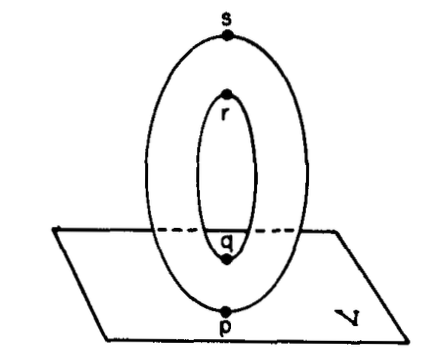
\includegraphics[width=0.4\linewidth]{resources/Diagram1.png}
    \label{fig:diagram1}
\end{figure}
Let $f: M \rightarrow \mathbb{R}$ be the distance of a point to the plane $V$. 
For a Number $a \in \mathbb{R} $, let $M^a$ be the set of all points $p \in M$, s.th. $f(p) \leq a$.
Then the following are true:
\begin{enumerate}
   \item[(1)] If $a < 0 < f(p)$, then $M^a = \varnothing$
   \item[(2)] If $f(p) < a < f(q)$, then $M^a$ is homeomorphic to a 2-cell.
   \item[(3)] If $f(q) < a < f(r)$, then $M^a$ is homeomorphic tp a cylinder.
   \item[(4)] If $f(q) < a < f(r)$, then $M^a$ is homeomorphic to a compact manifold of genus one with a circle as a boundary.
   \item[(5)] If $f(s) < a$, then $M^a = M$.
\end{enumerate}

To describe how $M^a$ changes as it passes through the points $f(p)$, $f(q)$, $f(r)$, $f(s)$ it is conveniant to consider
homotopy type rather than homeomorphism type. 
\begin{enumerate}[leftmargin=2cm]
   \item[(1) $\rightarrow$ (2)]: In case (1), $M^a$ has the same homotopy type as a point, so this step is the attaching of a 0-cell. 
   \item[(2) $\rightarrow$ (3)]: Is the operation of attaching a 1-cell. 
   \item[(3) $\rightarrow$ (4)]: Again is the operation of attaching a 1-cell. 
   \item[(4) $\rightarrow$ (5)]: Is the operation of attaching a 2-cell. 
\end{enumerate}

The definition of attaching a k-cell can be given as follows: \\
Let $S^k = \{x \in \mathbb{R}^{k+1} : \lVert x \rVert = 1\}$ be the $k$-sphere \\
and $D^k = \{ x \in \mathbb{R}^k : \lVert x \rVert \leq 1 \}$ be the $k$-disk.

Let $M$ and $N$ be manifolds, then $N$ is created from $M$ by atteching a k-cell,
if $N$ is of the same homotopy type as a topological space $X$ s.th. there exists 
a pushout square in Top

\begin{figure}[H]
   \centering
   \begin{tikzcd}
      S^{k-1} \arrow[r] \arrow[d] \arrow[dr, phantom, "\ulcorner", very near end] & M \arrow[d] \\
      D^k \arrow[r]                                                               & X
   \end{tikzcd}
\end{figure}

A pushout square in a category $\mathcal{C}$ is a commutative square 

\begin{figure}[H]
   \centering
   \begin{tikzcd}
      A \arrow[r, "f_0"] \arrow[d, "f_1"] & B \arrow[d, "g_0"] \\
      C \arrow[r, "g_0"]                  & D 
   \end{tikzcd}
\end{figure}      
   
s.th if there is another commutative diagram

\begin{figure}[H]
   \centering
   \begin{tikzcd}
      A \arrow[r, "f_0"] \arrow[d, "f_1"] & B \arrow[d, "h_0"] \\
      C \arrow[r, "h_1"]                  & \tilde{D}
   \end{tikzcd}
\end{figure}

Then 

\begin{figure}[H]
   \centering
   \begin{tikzcd}
      A \arrow[r, "f_0"] \arrow[d, "f_1"] & B \arrow[d, "g_0"] \arrow[rdd, "h_0", bend left] & \\
      C \arrow[r, "g_1"] \arrow[drr, "h_1", bend right] & D & \\
        &   & \tilde{D} \arrow[ul, "\exists!h", dashed]
   \end{tikzcd}
\end{figure}

which commutes everywhere.

\subsection{Definitions and Lemmas}

\begin{definition}[critical Point, non-degenerate critical Point]
   \label{def:critical point}

   Let $M$ be a (smooth) manifold and $f: M \rightarrow \mathbb{R}$ be a smooth function.
   Then $p \in M$ is called a \textit{critical point}, if the tangent map 
   $f_*: TM_p \rightarrow R$ is not zero. \\
   A critical point is called \textit{non-degenerate}, if for some local coordinates $\varphi = (x_1, ..., x_n)$
   the matrix 
   \[ H_p^{\varphi}f := \left(\frac{\partial^2 f}{\partial x_i \partial x_j}(p)\right)_{1 \leq i,j \leq n} \]
   is non-singular, i.e. invertable. \\
   $H_p^{\varphi}f$ is called the Hessian of $f$ at $p$ (wrt. $\varphi$).

\end{definition}

\begin{lemma}[Congruency of Hessians]
   \label{lemma:congruency}   

   Let $M$ be a manifold, $f: M \rightarrow \mathbb{R}$, $p$ a critical point of $f$
   and $\varphi := (x_1, ..., x_n)$ and $\psi := (y_1, ..., y_n)$ local coordinates
   aroud $p$. Let 
   \[ D_p = \left( \frac{\partial x_i}{\partial y_j}(p) \right)_{1 \leq i, j \leq n}\].
   Then 
   \[ H_p^{\psi}f = D_p^T H_p^{\varphi}f D_p \]

\end{lemma}

\begin{proof}

   Let $M$ be a manifold, $f: M \rightarrow \mathbb{R}$ a smooth function.
   Let $p \in M$ be a critical point of $f$ and $\varphi = (x_1, ..., x_n)$, $\psi = (y_1, ..., y_n)$
   local coordinates in a nbhd. around $p$.
   From functoriality of the tangent space, we know that 
   \[ \frac{\partial f}{\partial y_k} = \sum_{i=1}^n \frac{\partial f}{\partial x_i} \cdot \frac{\partial x_i}{\partial y_k} \]
   , so 

   \[ \pdderive[f]{y_k}{y_l} (p) 
   = \pderive{y_k} \left( \pderive[f]{y_l} \right) (p) 
   = \pderive{y_k} \left( \sum_{i=1}^n \pderive[f]{x_i} \cdot \pderive[x_i]{y_l} \right) (p) \]
   \[ = \sum_{i=1}^n \pderive{y_k} \left( \pderive[f]{x_i} \right) (p) \cdot \pderive[x_i]{y_l} (p) 
   + \sum_{i=1}^n \pderive[f]{x_i} (p) \cdot \pderive{y_k} \left( \pderive[x_i]{y_l} \right) (p) \]
   \[ = \sum_{i,j = 1}^n \pdderive[f]{x_i}{x_j} (p) \cdot \pderive[x_j]{y_k} (p) \cdot \pderive[x_i]{y_l}(p)
   + \sum_{i=1}^n \pderive[f]{x_i} (p) \cdot \pdderive[x_i]{y_k}{y_l}(p)\]
   
   Because $p$ is a critical point, $\pderive[f]{x_i} (p) = 0$ for all $i$, so then
   \[ \left( H_p^{\psi}f \right)_{k,l} = \sum_{i,j = 1}^n \pdderive[f]{x_i}{x_j} (p) \cdot \pderive[x_j]{y_k}(p) \cdot \pderive[x_i]{y_l} (p) \]
   \[ = \left( D_p^T \cdot H_p^{\varphi}f \cdot D_p \right)_{k,l} \]

\end{proof}

\begin{lemma}[Invariance of non-degeneracy] 
   \label{lemma:non-degeneracy}
   Non-degeneracy does not depend on the chosen local coordinates.
\end{lemma}

\begin{proof}
   Let $f: M \rightarrow \mathbb{R}$ be smooth, $p$ a critical point of $f$ and $\varphi = (x_1, ..., x_n)$, $\psi = (y_1, ..., y_n)$ 
   local coordinates around $p$. Assume that $p$ is non-non degenerate wrt. $\varphi$ Note that $D_p$ from lemma~\ref{lemma:congruency} is invertable. Then
   \[ \text{det}(H_p^{\psi}f) = \text{det}(D_p^T \cdot H_p^{\varphi} \cdot D_p) = \text{det}(D^T) \cdot \text{det}(H_p^{\varphi}) \cdot \text{det}(D_p) \neq 0 \]
\end{proof}

\begin{definition}[Index]
   \label{def:index}

   The \textit{index} of a Matrix $A$ is the number of (not necessarily destinct) negative Eigenvalues of $A$ and is denoted by
   $\text{index}(A)$. \\ The \textit{index} of a critical point $p$ of a function $f: M \rightarrow \mathbb{R}$ (wrt. a chart $\varphi$)
   is the index of the matrix $H_p^{\varphi}f$.
\end{definition}

\begin{lemma}[Invariance of the Index]
   \label{lemma:index}
   The index of a critical point does not depend on the chosen local coordinates.
\end{lemma}

\begin{proof}
   Let $f: M \rightarrow \mathbb{R}$ be a smooth function, $p$ a critical point of $f$
   and $\varphi$, $\psi$ two charts around $p$.
   As seen in lemma~\ref{lemma:congruency}, $H_p^{\varphi}f = D^T \cdot H_p^{\psi}f \cdot D$, i.e.
   $H_p^{\varphi}$ is congruent to $H_p^{\psi}$, because $D$ is invertable. Then by Sylvester's Law, 
   \[ \text{{index}}(H_p^{\varphi}f) = \text{{index}}(H_p^{\varphi}f) \]
\end{proof}

\begin{theorem}[Morse's Lemma]
   \label{theorem:morse lemma}

   Let $M$ be a manifold, $f: M \rightarrow \mathbb{R}$ smooth and $p$ a non-degenerate 
   critical point of $f$ of index $k$. Then there exist local coordinates $\varphi = (x_1, ..., x_n)$, s.th,
   \[ f = f(p) - x_1^2 - ... - x_k^2 + x_{k+1}^2 + ... + x_n^2 \]
\end{theorem}

\begin{proof}
   This is the proof of Morse's Lemma <3 . It's true i swear
\end{proof}

\begin{definition}[Morse Function]
   \label{def:morse function}

   Let $M$ be a manifold, $f:M \rightarrow \mathbb{R}$ a smooth map. $f$ is called a \textit{Morse Function},
   if all critical values of $f$ are non-degenerate.   
\end{definition}

\subsection{Homotopy Type in Terms of critical Values}

\begin{theorem}[First deformation Lemma]
   \label{theorem:1st deformation lemma}
   Let $M$ be a manifold, $f: M \rightarrow \mathbb{R}$ smooth. Let $a < b \in \mathbb{R}$, s.th. 
   $f^{-1}[a, b]$ is compact and contains no critical points of $f$. Then $M^a$ is diffeomorphic
   to $M^b$. \\ 
   Furthermore, $M^a$ is a nbhd. deformation retract of $M^b$, s.th. the inclusion
   $M^a \rightarrow M^b$ is a homotopy equivalence.
\end{theorem}

\begin{proof}
   Also the first deformation lemma is true, really
\end{proof}

\begin{theorem}[Second deformation Lemma]
   \label{theorem:2nd deformation lemma}
   Let $M$ be a manifold, $f: M \rightarrow \mathbb{R}$ smooth and $p$ be a non-degenerate critical point
   of $f$ of index $k$. Let $c := f(p)$ and $\epsilon > 0$, s.th. $f^{-1}[c-\epsilon, c+\epsilon]$
   is compact and contains no critical points of $f$. Then $M^{c+\epsilon}$ is obtained from $M^{c-\epsilon}$
   by attaching a $k$-cell.
\end{theorem}

\begin{proof}
   I'm not so sure if this is true but i guess
\end{proof}

\subsection{Examples}

\subsection{The Morse Inequalities}

\begin{lemma}[Weak morse Inequalities]
   \label{lemma:weak morse inequalities}

\end{lemma}

\begin{proof}


\end{proof}

\begin{lemma}[Strong morse Inequalities]
   \label{lemma:strung morse inequalities}

\end{lemma}

\begin{proof}

\end{proof}

\end{document}
